\newpage
\subsection{Ερώτημα ii}

\begin{tcolorbox}
Για την μελέτη των χαρακτηριστικών εκτελέσαμε τα 12 παραπάνω benchmarks για τους
συνδυασμούς χαρακτηριστικών επεξεργαστή που αναφέρθηκαν στο προηγούμενο ερώτημα.
Ωστόσο, πρέπει σε αυτό το σημείο να σημειώσουμε ότι ορισμένα από τα benchmarks
εμφάνιζαν errors κατά την εκτέλεση με αποτέλεσμα η προσομοίωση να εκτελείται για
μικρό αριθμό εντολών, γεγονός που σημαίνει ότι δεν είναι αξιόπιστη η "εικόνα"
της προσομοίωσης αυτής.
Λαμβάνοντας υπ' όψιν βάσει της εκφώνησης της εργαστηριακής άσκησης ότι το κάθε
pinball περιέχει περίπου 1 billion εντολές, και βάσει των αποτελεσμάτων στα
αρχεία sim.out βρέθηκε για το κάθε benchmark ότι εκτελούνται τα παρακάτω ποσοστά
εντολών: 


\begin{center}
   \vspace{3mm}
   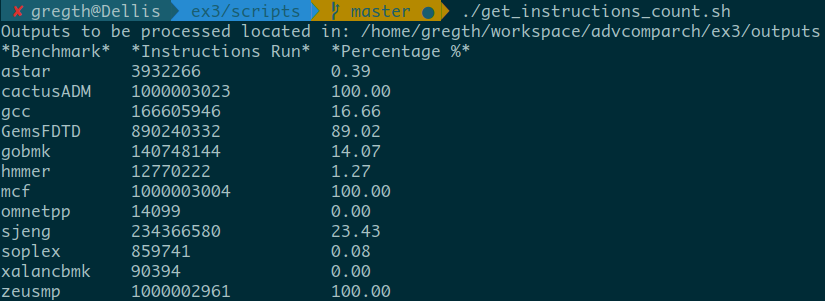
\includegraphics[width= \textwidth]{./imgs/count.png}
   \vspace{2mm}
\end{center}

Από τα benchmarks αυτά, και βάσει τον διευκρινήσεων που δόθηκαν θα κρατήσουμε 
τις προσμοποιώσεις οπου έχει εκτελεστεί παραπάνω από το 10 \% του pinball.
Συνεπώς, δεν έχει νόημα να μελετήσουμε 5 από τα 12 benchmarks,
και συγκεκριμένα τα astar, hmmer, soplex, xalancbmk, omnetpp.

\end{tcolorbox}

\noindent \\Ακολουθούν τα διαγράμματα και ο σχολιασμός τους:

\vspace{3mm}
   \begin{minipage}{\textwidth}
      \begin{center}
         \fbox{\textlatin{\textbf{\textit{403-gcc}}}}\\
         \vspace{3mm}
         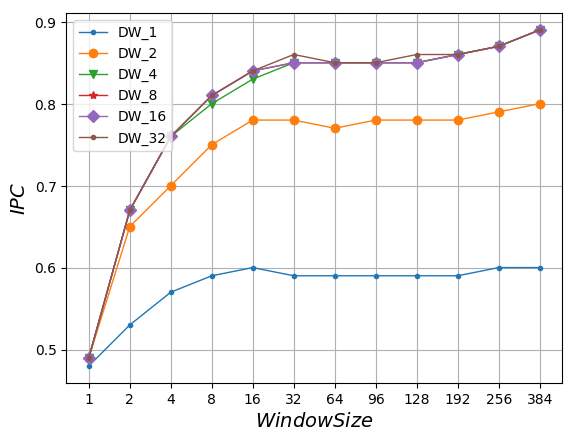
\includegraphics[width=0.7\textwidth, frame]{./graphs/ipc/gcc.png}
         \vspace{6mm}
      \end{center}
   \end{minipage}

   \begin{minipage}{\textwidth}
      \begin{center}
         \fbox{\textlatin{\textbf{\textit{429-mcf}}}}\\
         \vspace{3mm}
         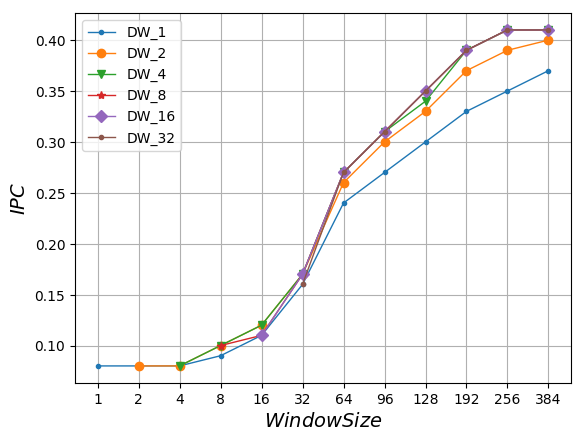
\includegraphics[width=0.7\textwidth, frame]{./graphs/ipc/mcf.png}
         \vspace{6mm}
      \end{center}
   \end{minipage}

   \begin{minipage}{\textwidth}
      \begin{center}
         \fbox{\textlatin{\textbf{\textit{434-zeusmp}}}}\\
         \vspace{3mm}
         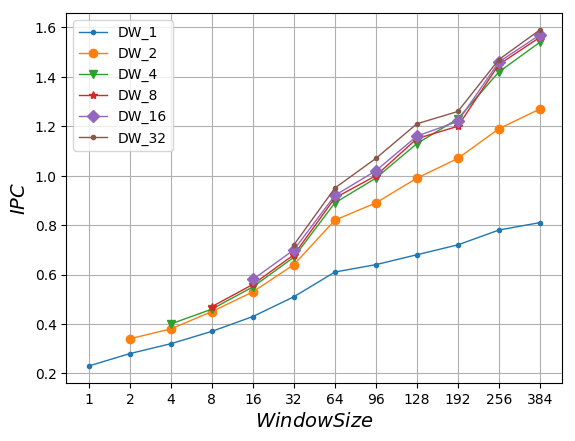
\includegraphics[width=0.7\textwidth, frame]{./graphs/ipc/zeusmp.png}
         \vspace{6mm}
      \end{center}
   \end{minipage}

   \begin{minipage}{\textwidth}
      \begin{center}
         \fbox{\textlatin{\textbf{\textit{436-cactusADM}}}}\\
         \vspace{3mm}
         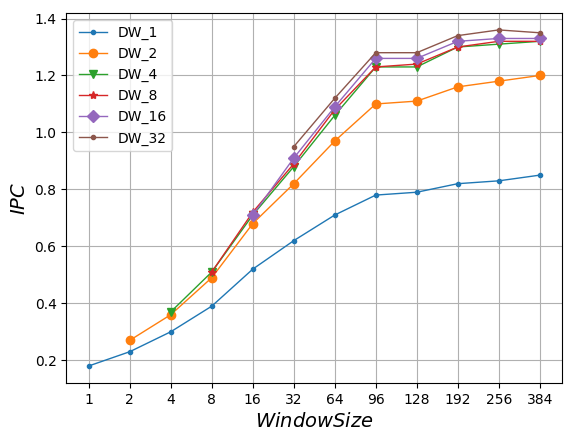
\includegraphics[width=0.7\textwidth, frame]{./graphs/ipc/cactusADM.png}
         \vspace{6mm}
      \end{center}
   \end{minipage}

   \begin{minipage}{\textwidth}
      \begin{center}
         \fbox{\textlatin{\textbf{\textit{445-gobmk}}}}\\
         \vspace{3mm}
         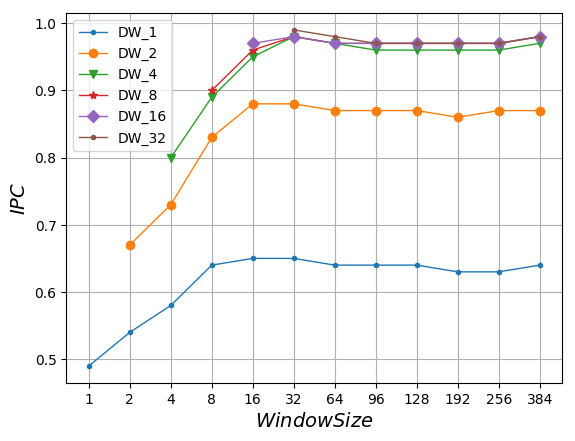
\includegraphics[width=0.7\textwidth, frame]{./graphs/ipc/gobmk.png}
         \vspace{6mm}
      \end{center}
   \end{minipage}

   \begin{minipage}{\textwidth}
      \begin{center}
         \fbox{\textlatin{\textbf{\textit{458-sjeng}}}}\\
         \vspace{3mm}
         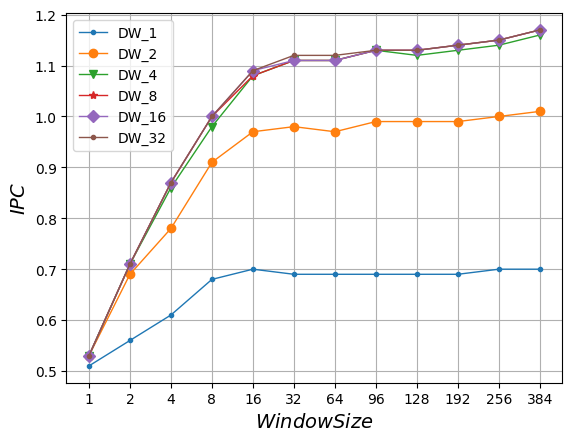
\includegraphics[width=0.7\textwidth, frame]{./graphs/ipc/sjeng.png}
         \vspace{6mm}
      \end{center}
   \end{minipage}

   \begin{minipage}{\textwidth}
      \begin{center}
         \fbox{\textlatin{\textbf{\textit{459-GemsFDTD}}}}\\
         \vspace{3mm}
         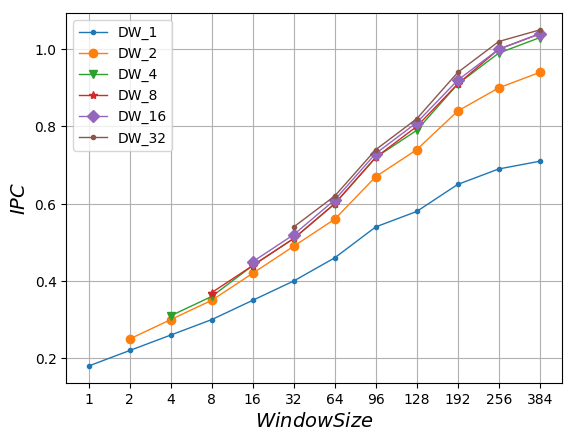
\includegraphics[width=0.7\textwidth, frame]{./graphs/ipc/GemsFDTD.png}
         \vspace{6mm}
      \end{center}
   \end{minipage}


   \paragraph{Συμπεράσματα - Σχόλια}
   Από τις παραπάνω γραφικές του IPC συναρτήσει των dispatch width και window
   size μπορούμε εύκολα να συμπεράνουμε ότι η αύξηση του dispatch width από 1 σε
   2 και από 2 σε 4 εντολές επιφέρει σημαντική βελτίωση της επίδοσης. Ωστόσο,
   περαιτέρω αύξηση σε του dispatch width σε 8, 16 ή και 32 εντολές δεν επιφέρει
   σημαντική αλλαγή στην επίδοση (οι γραφικές για τις τιμές αυτές είναι ως επί
   το πλείστον επικαλυπτόμενες) και άρα δεν έχει νόημα. Αυτό μπορεί να
   ερμηνευθεί λόγω των περιορισμών του ILP (Instruction Level Parallelism) του
   κώδικα που εκτελείται. Δηλαδή, είναι δύσκολο να υπαρξουν και να γίνουν issue
   μεγάλες πλειάδες εντολών (κάθε πλειάδα πάνω από 4 εντολές) που να είναι
   ανεξάρτητες μεταξύ τους ώστε να μπορούν να γίνουν process παράλληλα και να
   επιτύχουμε με ικανοποιητικό ipc. 


   Όσον αφορά το window size, δηλαδή το μέγεθος του Reorder Buffer, βλέπουμε πως
   καθώς αυξάνεται, αυξάνεται συνήθως και το ipc. Αναλυτικότερα, υπάρχουν
   benchmarks (gemsFDTD, cactusADM, zeusmp, mcf)  που αυτή η αύξηση συνεχίζεται
   διαρκώς καθώς αυξάνεται το μέγεθος του ROB, λαμβάνοντας μέγιστη τιμή για το
   μεγαλύτερο window size = 384 και άλλα benchmarks (sjeng, gobmk, gcc) για τα
   οποία η αύξηση είναι σημαντική (μεγάλη κλίση) μέχρι ενός ορίου windows size =
   32 με 64 περίπου, και από το σημείο αυτό και πέρα η αύξηση του ipc δεν είναι
   τόσο σημαντική (μικρότερη κλίση).
   
   Αξίζει επίσης να σημειώσουμε ότι στα benchmarks zeusmp, cactusADM, sjeng,
   GemsFDTD το IPC καταφέρνει να ξεπεράσει τη μονάδα για dispatch width = 4 και
   αρκούντως μεγάλο window size.

   Βάσει των παραπάνω, για την κατασκευή θα επιλέγαμε πιθανότατα dispatch width =
   4 (ή εναλλακτικά 8) και ένα αρκετά μεγάλο window size, το οποίο θα μας υπαγόρευαν άλλοι
   περιορισμοί, όπως η ενέργεια και το κόστος.